%! Author = Adrian Helberg
%! Date = 20.10.2020

% Preamble
\documentclass[12pt]{beamer}
\usetheme{Marburg}
\usepackage{ngerman}
\usepackage{graphicx}
\usepackage{tikz}
\usepackage{wrapfig}

\title{Arbeitspakete}
\author{Adrian Helberg}
\date{\today}

% Document
\begin{document}
    \maketitle

    \section{Arbeitspaket 1}
    \label{sec:1}

    \begin{frame}
        \frametitle{Arbeitspaket 1}
        Hier soll die Benutzerschnittstelle erstellt werden.
        Es umfasst die Bereiche:
        \begin{itemize}
            \item[I.] Strukturieren
            \item[II.] Visualisieren
        \end{itemize}
    \end{frame}

    \begin{frame}
        \frametitle{Beschreibung}
        \begin{itemize}
            \setlength\itemsep{1em}
            \item Der Benutzer des Systems nutzt die Benutzerschnittstelle, um eine Verzweigungsstruktur zu erstellen
            \item Ziel ist die Weitergabe der erstellten Struktur mit Informationen wie Topologie und Transformationen an den
            nächsten Arbeitsschritt
        \end{itemize}
    \end{frame}

    \begin{frame}[fragile]
        \frametitle{Ablauf}
        Das Programm soll folgenden Workflow umsetzen:\\~\\
        \begin{itemize}
            \item[1] Erster Anker ist vorselektiert
            \item[2] Widerhole, bis Struktur erstellt ist:
            \begin{itemize}
                \item[2.1] Selektiere ein Template aus der Liste
                \item[2.2] Setze Parameter
                \item[2.3] Bestätige Auswahl und Parameter
                \item[2.4] Zeichne ausgewähltes Template mit Parametern
                \item[2.5] Wähle nächsten Anker aus
            \end{itemize}
        \end{itemize}
    \end{frame}

    \begin{frame}[fragile]
        \frametitle{Schlüsselwörter}
        \begin{figure}
            \centering
            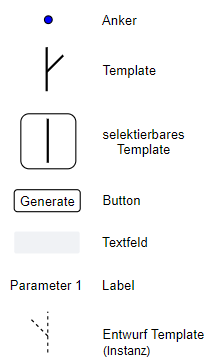
\includegraphics[width=3cm]{../images/UI_Legende.PNG}
            \caption{Legende}
        \end{figure}
    \end{frame}

    \begin{frame}
        \frametitle{Beispiel}
        \begin{figure}
            \centering
            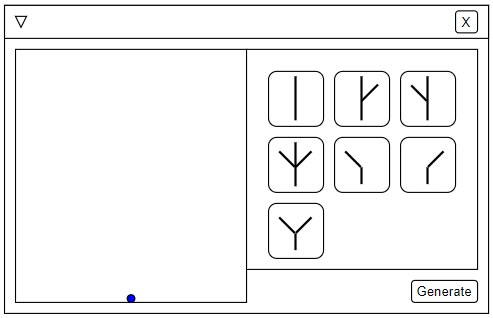
\includegraphics[width=4cm]{../images/UI_1.PNG}
            \caption{Erster Anker ist vorselektiert}
        \end{figure}
        \begin{figure}
            \centering
            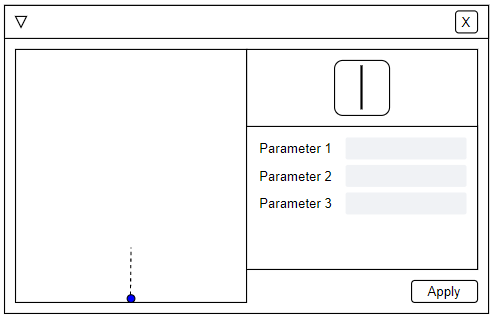
\includegraphics[width=4cm]{../images/UI_2.PNG}
            \caption{Setze Parameter (1/2)}
        \end{figure}
    \end{frame}

    \begin{frame}
        \frametitle{Beispiel}
        \begin{figure}
            \centering
            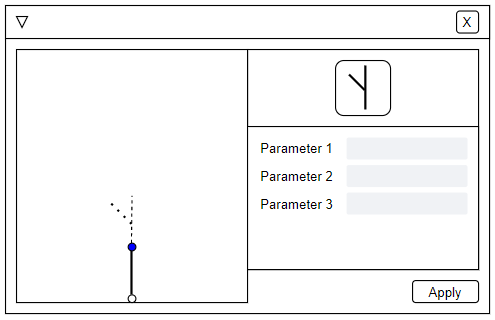
\includegraphics[width=4cm]{../images/UI_4.PNG}
            \caption{Setze Parameter (2/2)}
        \end{figure}
        \begin{figure}
            \centering
            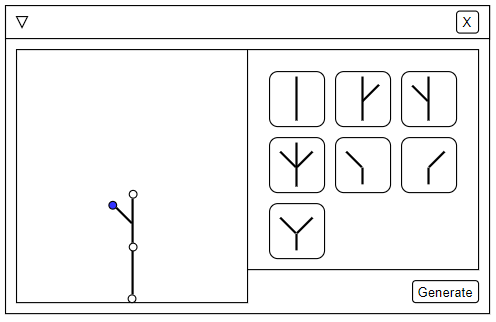
\includegraphics[width=4cm]{../images/UI_5.PNG}
            \caption{Zeichne Template nach Bestätigung (\textit{apply})}
        \end{figure}
    \end{frame}

    \begin{frame}
        \frametitle{Beispiel}
        \begin{figure}
            \centering
            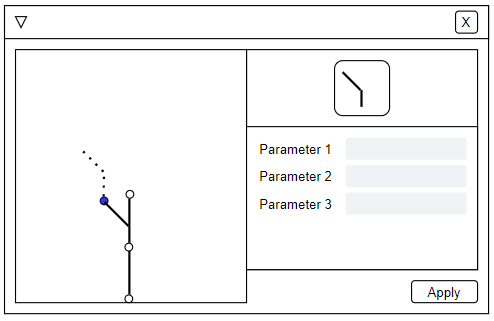
\includegraphics[width=4cm]{../images/UI_6.PNG}
            \caption{Selektierter Anker 1}
        \end{figure}
        \begin{figure}
            \centering
            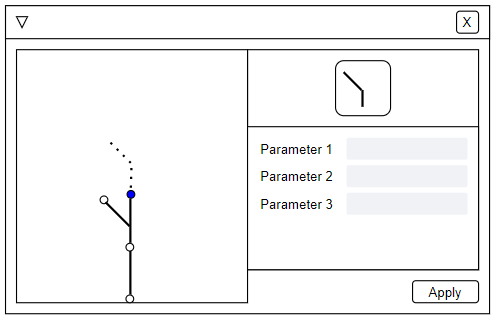
\includegraphics[width=4cm]{../images/UI_7.PNG}
            \caption{Selektierter Anker 2}
        \end{figure}
    \end{frame}

    \section{Arbeitspaket 2}
    \label{sec:2}

    \begin{frame}
        \frametitle{Arbeitspaket 2}
        Hier soll eine Baumstruktur aufgebaut werden.
        Es umfasst die Bereiche:
        \begin{itemize}
            \item[III.] Datengenerierung
        \end{itemize}
    \end{frame}

    \begin{frame}
        \frametitle{Beschreibung}
        \begin{itemize}
            \item \textbf{Templates} sind beliebige, atomare Verzweigungsstrukturen
            \item \textbf{Instanzen} sind transformierte Templates (z.B. skalierte, rotierte Templates)
            \item Die in Arbeitspaket 1 erstellte Struktur stellt eine Sammlung von verknüpften Template-Instanzen dar
        \end{itemize}
    \end{frame}

    \begin{frame}
        \frametitle{Beschreibung}
        \textit{Topologie und Transformation der Struktur sollen in einer  Baumstruktur organisiert werden:}
        \begin{itemize}
            \item \textbf{Knoten} entprechen Instanzen
            \item \textbf{Kanten} verknüpfen Eltern-Knoten mit ihren Kind-Knoten und stellen Parameter wie Rotation
            und Skalierung (relativ zum Eltern-Knoten) dar
            \item \textbf{Blätter} sind Instanzen ohne Kindknoten
            \item Jeder Kindknoten hate \underline{genau} einen Elternknoten, also eine eingehende Kante, und n
            Kindknoten, also n ausgehende Kanten
        \end{itemize}
    \end{frame}

    \begin{frame}
        \frametitle{Baum}
        Der resultierende Baum ist ein Wurzelbaum (Syntaxbaum):\\~\\
        \textit{Der Baum ist ein gerichteter, geordneter, azyklischer Graph, in dem genau ein Knoten $w$ Eingangsgrad 0
        besitzt und alle anderen Knoten Eingangsgrad 1 besitzen. Knoten $w$ heißt die Wurzel des Graphen}
    \end{frame}

    \begin{frame}
        \frametitle{Beispiel - Templates}
        \begin{figure}
            \centering
            
\includegraphics[width=0.3cm]{../images/Template_4.PNG}
            
\includegraphics[width=1.1cm]{../images/Template_1.PNG}
            \\~\\
            
\includegraphics[width=0.6cm]{../images/Template_2.PNG}
            
\includegraphics[width=0.6cm]{../images/Template_3.PNG}
        \end{figure}
    \end{frame}

    \begin{frame}
        \frametitle{Struktur}
        \begin{columns}
            \begin{column}{0.5\textwidth}
                \begin{figure}
                    \centering
                    \begin{tikzpicture}
                        \node (w) at (0,0) [circle, shade, draw] {$w$};
                        \node (a) at (0,-1.5) [circle, draw] {
\includegraphics[width=0.1cm]{../images/Template_4.PNG}};
                        \node (b) at (0,-3) [circle, draw] {
\includegraphics[width=0.3cm]{../images/Template_1.PNG}};
                        \node (c) at (-1.5,-4.5) [circle, draw] {
\includegraphics[width=0.2cm]{../images/Template_2.PNG}};
                        \node (d) at (0,-4.5) [circle, draw] {
\includegraphics[width=0.1cm]{../images/Template_4.PNG}};
                        \node (e) at (1.5,-4.5) [circle, draw] {
\includegraphics[width=0.2cm]{../images/Template_3.PNG}};
                        \node (f) at (1,-6) [circle, draw] {
\includegraphics[width=0.2cm]{../images/Template_2.PNG}};
                        \node (g) at (2,-6) [circle, shade, draw] {$x$};
                        \draw [->, thick] (w) to (a);
                        \draw [->, thick] (a) to (b);
                        \draw [->, thick] (b) to (c);
                        \draw [->, thick] (b) to (d);
                        \draw [->, thick] (b) to (e);
                        \draw [->, thick] (e) to (f);
                        \draw [->, thick] (e) to (g);
                    \end{tikzpicture}
                \end{figure}
            \end{column}
            \begin{column}{0.5\textwidth}
                \begin{figure}
                    \centering
                    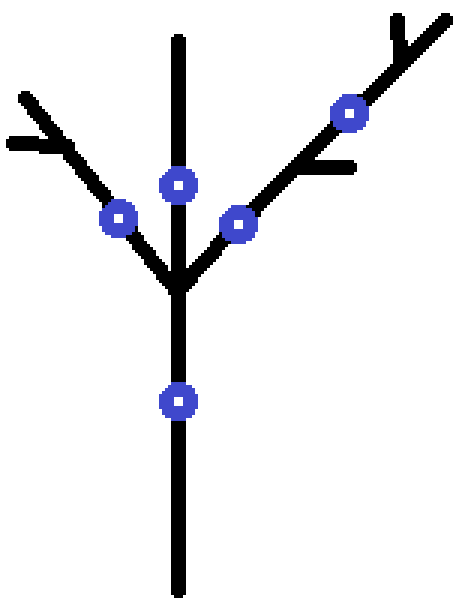
\includegraphics[width=4cm]{../images/Tree_1.PNG}
                \end{figure}
            \end{column}
        \end{columns}
    \end{frame}

    \section{Arbeitspaket 3}
    \label{sec:3}

    \begin{frame}
        \frametitle{Arbeitspaket 3}
        Hier soll ein "`kleines"'\footnote{Smallest Grammar Problem} L-System, das \underline{nur} die Input-Struktur beschreibt aus der
        Baumstruktur
        inferiert werden Es umfasst die Bereiche:
        \begin{itemize}
            \item[IV.] Inferieren
        \end{itemize}
    \end{frame}

    \begin{frame}
        \frametitle{Überlegungen}
        \begin{figure}
            \centering
            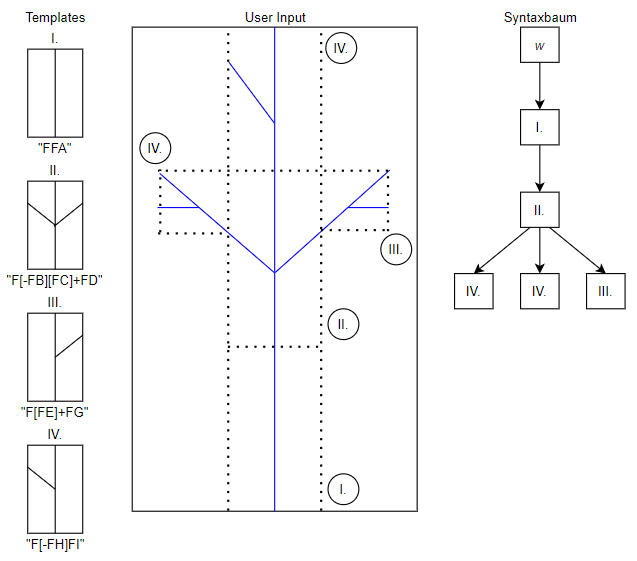
\includegraphics[width=8cm]{../images/Beispiel_1.PNG}
            \caption{Beispiel}
        \end{figure}
    \end{frame}

    \begin{frame}
        \frametitle{Kompaktes L-System aufbauen}
        $L = \{V, S, w, P\}$ mit
        \begin{itemize}
            \item $V$ als alle nicht-terminalen Symbole
            \item $S$ als alle terminalen Symbole
            \item $w$ als Axiom (Startwort)
            \item $P$ als Menge von Produktionsregeln (geordnete Paare bsp. $A \rightarrow X$ mit $X$ aus $V \cup S$
            (Alphabet))
        \end{itemize}
    \end{frame}

    \begin{frame}
        \frametitle{Kompaktes L-System aufbauen}
        $L = \{M, \omega, R\}$ mit
        \begin{itemize}
            \item $M$ als Menge von Modulen (bsp. $A(P)$ mit $P$ als Liste von Parametern)
            \item $w$ als Axiom (Startwort)
            \item $R$ als Menge von Produktionsregeln
        \end{itemize}
    \end{frame}

    \begin{frame}
        \frametitle{Ablauf 1/2}
        \textit{Initialisierung:}
        \begin{itemize}
            \item[1.] Alphabet $M=\{F,S\}$, Regelmenge $R=\emptyset$, Axiom $\omega=S$
            \item[2.] Füge neue Regel $\alpha$: $S \rightarrow A$ der Regelmenge $R$ hinzu
            \item[3.] Knoten $\beta=$ nächster Knoten\footnote{nach Breitensuche, beginnend bei Wurzelknoten S}
            \item[4.] Füge nächstes Symbol $\gamma$ aus $\{A,B,\dots,Z\}$, das nicht in $M$ enthalten ist, zu $M$ hinzu
        \end{itemize}
    \end{frame}

    \begin{frame}
        \frametitle{Ablauf 2/2}
        \textit{Schleife:}
        \begin{itemize}
            \item[5.] Wiederhole:
            \begin{itemize}
                \item[a.] Wort $\delta=$ Wort von $\beta$
                \item[b.] Für alle Symbole $\{X,Y,Z\}$ aus $\delta$
                \begin{itemize}
                    \item[I.] Ersetze Symbol mit neuem Symbol, das nicht in $M$ enthalten ist und füge es $M$ hinzu
                \end{itemize}
                \item[d.] Füge $\gamma\rightarrow\delta$ der Regelmenge $R$ hinzu
                \item[e.] Wenn es ein Symbol in $M\setminus\{F,S\}$ gibt, für das es keine Regel gibt, dann:
                \begin{itemize}
                    \item $\gamma=$ nächstes Symbol aus $M$, für das es keine Regel gibt
                \end{itemize}
                \item[f.] Ansonsten:
                \begin{itemize}
                    \item Breche \textit{Schleife} ab
                \end{itemize}
                \item[g.] $\beta=$ nächster\footnote{nach Breitensuche, beginnend bei Wurzelknoten S} Knoten
            \end{itemize}
        \end{itemize}
    \end{frame}

    \section{Arbeitspaket 4}
    \label{sec:4}

    \begin{frame}
        \frametitle{Beschreibung}
        Arbeitspaket 4
    \end{frame}

    \section{Arbeitspaket 5}
    \label{sec:5}

    \begin{frame}
        \frametitle{Beschreibung}
        Arbeitspaket 5
    \end{frame}

\end{document}